\chapter{第一代量子天文学科学案例}
\label{chap:19}

\begin{chapteropening}
第一代科学案例要同时满足光子率、角尺度、基线覆盖、校准难度和失败后仍有用的科学产出。强度干涉已经从 Sirius 和 Narrabri 的亮星角直径，发展到 VERITAS、MAGIC、Vega photon-counting 和新近的快速自转星测量；这些结果把起点指向明亮、热、小角尺度、外部先验充足的目标。恒星角直径、快速自转、密近双星、Be/WR 谱线区、新星早期膨胀、Crab 光子统计和自然激光候选，构成第一批最现实的项目清单 \citep{1956Natur.178.1046H,1974MNRAS.167..121H,2006ApJ...649..399L,2012NewAR..56..143D,2020NatAs...4.1164A,2020MNRAS.491.1540A,2021MNRAS.506.1585Z,2024MNRAS.529.4387A}。
\end{chapteropening}

\section{案例排序从哪三个坐标开始}

亮度是第一道门槛。对当前强度干涉，\(m_V\lesssim5\) 的热星是验证区，\(m_V\simeq6-7\) 是有挑战但可规划的区域，\(m_V\gtrsim9\) 通常需要更大阵列、多谱通道、长积分或更低系统噪声。Dravins 等给出的目标研究把亮热星、发射线结构和快速自转星列为自然起点；LeBohec--Holder 的估算也显示，一对 \(100\,{\rm m^2}\)、GHz 级电子带宽的望远镜在 5 h 内可对 \(m_V\simeq6.7\) 的源达到几 sigma 相关检出 \citep{2006ApJ...649..399L,2010SPIE.7734E..0AD,2012NewAR..56..143D,2013APh....43..331D}。

角尺度决定这些光子能否变成参数约束。若目标角尺度 \(\theta\) 远大于 \(\lambda/B\)，长基线上的 \(|V|^2\) 接近零，只有短基线有信号；若 \(\theta\) 远小于 \(\lambda/B\)，所有基线都看见未解析源，直径导数很小。第一代项目最好让主要结构落在 50--300 m 现有 IACT 基线或 0.5--2 km 未来 CTA 型基线上。外部先验也会改变可解释性：已知距离、光谱、轨道、径向速度、校准角直径或理论模型，会把 \(|V|^2\) 的少量数据点变成物理参数 \citep{2003RPPh...66..789M,2010SPIE.7734E..1CN,2010SPIE.7734E..1TJ,2012MNRAS.419..172N,2012MNRAS.424.1006N}。

\begin{figure}[tbp]
\centering
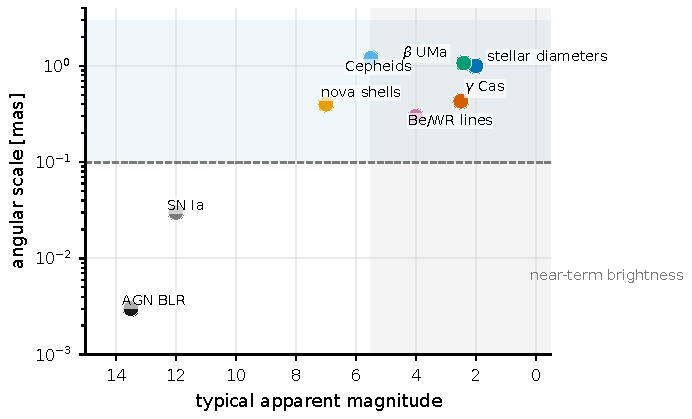
\includegraphics[width=0.88\linewidth]{figures/generated/chapter_19/ch19_science_case_feasibility.pdf}
\caption{第一代候选目标的亮度和角尺度位置。亮星角直径、\(\beta\) UMa、\(\gamma\) Cas 和 Be/WR 谱线区同时满足“够亮”和“能被百米级基线解析”；Type Ia、AGN BLR 和暗物质小尺度透镜科学价值高，但亮度、事件率或角尺度把它们推向长期项目。}
\label{fig:ch19-case-plane}
\end{figure}

一个实用排序分数可写成
\begin{equation}
  \mathcal P
  =
  \frac{
  W_{\rm sci}\,
  R_{\rm tech}\,
  R_{\rm prior}
  }{
  1+R_{\rm sys}+R_{\rm trigger}
  } .
  \label{eq:ch19-priority-score}
\end{equation}
\begin{formulaexplain}[公式 (19.1) 解读]
\(\mathcal P\) 是项目排序分数。科学回报、技术成熟度和外部先验提高分数；系统误差风险和触发风险降低分数，用来避免只凭“题目好听”选目标。
\end{formulaexplain}
\(W_{\rm sci}\) 是科学回报，\(R_{\rm tech}\) 是技术成熟度，\(R_{\rm prior}\) 是外部先验和模型可解释性，\(R_{\rm sys}\) 是系统误差风险，\(R_{\rm trigger}\) 是触发和调度风险。实际排序只需要粗分档，目的是防止单一维度支配选择。例如 Type Ia 几何距离的 \(W_{\rm sci}\) 很高，但 \(R_{\rm trigger}\) 和 \(R_{\rm tech}\) 也高；亮星角直径的 \(W_{\rm sci}\) 中等，却有很高 \(R_{\rm tech}\) 和低系统风险，适合做第一批验收指标 \citep{2025PhRvD.111h3047K,2024ApJ...966...28A,2024MNRAS.529.4387A}。

\section{恒星角直径、有效温度和快速自转为什么先做}

角直径是第一代最成熟的科学产品。观测量是 \(|V|^2(B,\lambda)\)，模型通常从均匀圆盘开始，再用 limb-darkened profile 或完整大气模型修正。角直径进入有效温度的方式很直接：
\begin{equation}
  F_{\rm bol}
  =
  \frac{\theta_{\rm LD}^2}{4}
  \sigma_{\rm SB}T_{\rm eff}^4,
  \qquad
  T_{\rm eff}
  =
  \left(
  \frac{4F_{\rm bol}}
  {\sigma_{\rm SB}\theta_{\rm LD}^2}
  \right)^{1/4}.
  \label{eq:ch19-teff}
\end{equation}
\begin{formulaexplain}[公式 (19.2) 解读]
\(F_{\rm bol}\) 是总辐射流量，\(\theta_{\rm LD}\) 是边缘昏暗角直径，\(T_{\rm eff}\) 是有效温度。角直径一旦测准，就能把流量转换成恒星温度尺度。
\end{formulaexplain}
\(F_{\rm bol}\) 是地球处总辐射流量，单位 \({\rm erg\,s^{-1}\,cm^{-2}}\)；\(\theta_{\rm LD}\) 是边缘昏暗角直径，单位 rad；\(\sigma_{\rm SB}\) 是 Stefan--Boltzmann 常数。若 \(\theta_{\rm LD}\) 误差为 \(4\%\)，只由角直径传播到 \(T_{\rm eff}\) 的误差约为 \(2\%\)。因此，亮星角直径重复测量不只是仪器复现实验；它会进入 \(T_{\rm eff}\)、半径、年龄、旋转模型和标准星尺度的校准 \citep{1967MNRAS.137..393H,1974MNRAS.167..121H,1977MNRAS.180..177B,1986Natur.323..234D,2003RPPh...66..789M}。

VERITAS-SII 已把这条路线推进到现代仪器。它对 \(\beta\) CMa 和 \(\epsilon\) Ori 给出亚毫角秒直径，并且比 Narrabri 用少得多的观测时间达到优于 \(5\%\) 的结果；后续 \(\beta\) UMa 观测在 416 nm 得到 limb-darkened 角直径 \(\theta_{\rm LD}=1.07\pm0.04_{\rm stat}\pm0.05_{\rm sys}\,{\rm mas}\)，与 CHARA 近红外和 Keck 中红外结果互相校验。MAGIC-SII 的升级系统报告了 22 个恒星直径，其中 9 个是参考星、13 个此前没有可比测量；强度干涉已经开始提供成批的角直径数据，而不再只是单次演示 \citep{2020NatAs...4.1164A,2024ApJ...966...28A,2024MNRAS.529.4387A}。

\Needspace{13\baselineskip}
快速自转星是角直径案例的自然升级。均匀圆盘只需要 \(\theta\)，椭圆 photosphere 至少需要短轴 \(\theta_{\rm min}\)、轴比 \(r=\theta_{\rm maj}/\theta_{\rm min}\) 和位置角 \(\varphi_\star\)。椭圆模型可以写成
\begin{equation}
  x_{\rm ell}
  =
  \frac{\pi B_p\theta_{\rm min}}{\lambda}
  \left[
  \cos^2\psi
  +
  r^2\sin^2\psi
  \right]^{1/2},
  \qquad
  |V_{\rm ell}|^2
  =
  \left[\frac{2J_1(x_{\rm ell})}{x_{\rm ell}}\right]^2 .
  \label{eq:ch19-elliptical-visibility}
\end{equation}
\begin{formulaexplain}[公式 (19.3) 解读]
\(x_{\rm ell}\) 是椭圆盘在当前投影基线上的无量纲空间频率，\(r\) 是轴比，\(\psi\) 是基线方向角。公式把快速自转星的扁形光球写成可拟合的 \(|V|^2\) 曲线。
\end{formulaexplain}
\(\psi\) 是投影基线相对短轴的角度。若基线位置角覆盖不足，\(r\) 和 \(\varphi_\star\) 会严重退化。VERITAS 对 \(\gamma\) Cas 的结果给出短轴角直径约 \(0.43\pm0.02_{\rm stat}\pm0.02_{\rm sys}\,{\rm mas}\)、轴比约 \(1.28\pm0.04\pm0.02\)、旋转轴位置角约 \(116^\circ\)，并用 Roche--von Zeipel 模型推断其接近 breakup rotation。第一代强度干涉已经能从“大小”推进到“形状”和“重力昏暗” \citep{2025ApJ...995..191A}。

\section{双星、Be 星盘和 Wolf-Rayet 风怎样用基线分开}

密近双星的好处是信号形状很有辨识度。两个未解析点源，角分离向量为 \({\bf s}\)，流量比为 \(f=F_2/F_1\)，则
\begin{equation}
  |V_{\rm binary}|^2
  =
  \left|
  \frac{1+f\,e^{-2\pi i{\bf u}\cdot{\bf s}}}
  {1+f}
  \right|^2
  =
  \frac{1+f^2+2f\cos(2\pi{\bf u}\cdot{\bf s})}
  {(1+f)^2}.
  \label{eq:ch19-binary-visibility}
\end{equation}
\begin{formulaexplain}[公式 (19.4) 解读]
\({\bf u}\) 是空间频率，\({\bf s}\) 是双星角分离，\(f\) 是流量比。指数相位带来随基线振荡的 \(|V|^2\)，所以强度干涉仍能约束双星分离。
\end{formulaexplain}
\({\bf u}={\bf B}_\perp/\lambda\)。当 \(f=1\) 时，\(|V|^2\) 会从 1 振荡到 0；当 \(f=0.1\) 时，振幅只有 \(2f/(1+f)^2\simeq0.17\)，对校准和 SNR 的要求高很多。双星项目最适合已有光谱轨道或食双星先验的系统；每个夜晚的少量基线点能被轨道模型连接起来，失败时也能给出分离或亮度比上限 \citep{1974MNRAS.167..121H,2012MNRAS.419..172N,2014MNRAS.437..798M,2022MNRAS.512.1722K}。

\begin{figure}[tbp]
\centering
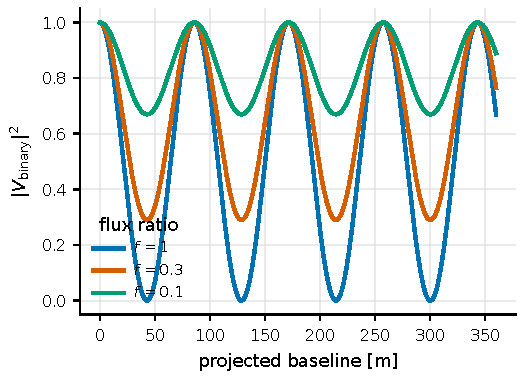
\includegraphics[width=0.82\linewidth]{figures/generated/chapter_19/ch19_binary_visibility.pdf}
\caption{1 mas 双星在 416 nm 下的平方可见度振荡。等亮双星给出深振荡；流量比降到 0.3 或 0.1 后，振荡振幅迅速变小。双星项目需要基线覆盖和轨道先验，否则亮度比、分离和位置角会互相退化。}
\label{fig:ch19-binary-visibility}
\end{figure}

\Needspace{12\baselineskip}
Be 星盘和 Wolf-Rayet 风把“空间分辨”与“谱线选择”连在一起。连续谱主要来自 photosphere，H\(\alpha\)、He 或 Fe 线可来自扩展盘、风碰撞区或 Weigelt blob 一类稠密结构。若谱线和连续谱混合，总可见度是通量加权和：
\begin{equation}
  V_{\rm obs}
  =
  \frac{
  F_{\rm c}V_{\rm c}
  +
  F_{\rm line}V_{\rm line}
  }{
  F_{\rm c}+F_{\rm line}
  } .
  \label{eq:ch19-line-continuum}
\end{equation}
\begin{formulaexplain}[公式 (19.5) 解读]
\(V_{\rm c}\) 和 \(V_{\rm line}\) 分别是连续谱和谱线区可见度，\(F_{\rm c}\) 与 \(F_{\rm line}\) 是对应通量。观测到的是通量加权平均，谱线几何必须和连续谱分开解释。
\end{formulaexplain}
\(F_{\rm line}/F_{\rm c}\) 可以从同时光谱或窄带/连续谱滤光片估计。若谱线区比 photosphere 大，长基线 \(|V_{\rm line}|^2\) 会比连续谱下降得更快；若谱线来自很小的高亮斑，长基线会保留信号。Narrabri 对 \(\gamma^2\) Velorum 的 WR 风已经展示了发射线区和连续谱区可以有不同角尺度；现代多基线阵列可把这一思想推广到 Be decretion disk、快速自转热星和相互作用双星 \citep{1970MNRAS.148..103H,2010SPIE.7734E..0AD,2012NewAR..56..143D,2025ApJ...995..191A}。

\section{新星、Type Ia 和可触发瞬变什么时候值得抢}

膨胀瞬变的几何关系简单，观测要求却很硬。若外壳以速度 \(v_{\rm exp}\) 近似自由膨胀，角直径为
\begin{equation}
  \theta(t)
  \simeq
  \frac{2v_{\rm exp}(t-t_0)}{D},
  \qquad
  D
  \simeq
  \frac{2v_{\rm exp}(t-t_0)}{\theta}.
  \label{eq:ch19-expansion}
\end{equation}
\begin{formulaexplain}[公式 (19.6) 解读]
\(\theta(t)\) 是膨胀外壳角直径，\(v_{\rm exp}\) 是膨胀速度，\(t_0\) 是爆发时刻，\(D\) 是距离。它是瞬变几何距离的最简账本。
\end{formulaexplain}
\(v_{\rm exp}\) 来自谱线速度，单位 \({\rm cm\,s^{-1}}\)；\(D\) 是距离；\(t-t_0\) 是爆发后时间。银河系新星在 \(D=2\,{\rm kpc}\)、\(v_{\rm exp}=10^8\,{\rm cm\,s^{-1}}\) 时，10 天后角直径已达数 mas，用百米以下基线即可解析；主要困难来自亮度演化、非球对称形状和尘埃。Type Ia 在 \(D=10\,{\rm Mpc}\)、\(v_{\rm exp}=10^9\,{\rm cm\,s^{-1}}\) 时，20 天后角直径只有 \(\sim0.02\,{\rm mas}\)，需要数 km 光学基线；限制它的主要是触发窗口、亮度和阵列规模 \citep{2025PhRvD.111h3047K}。

\begin{figure}[tbp]
\centering
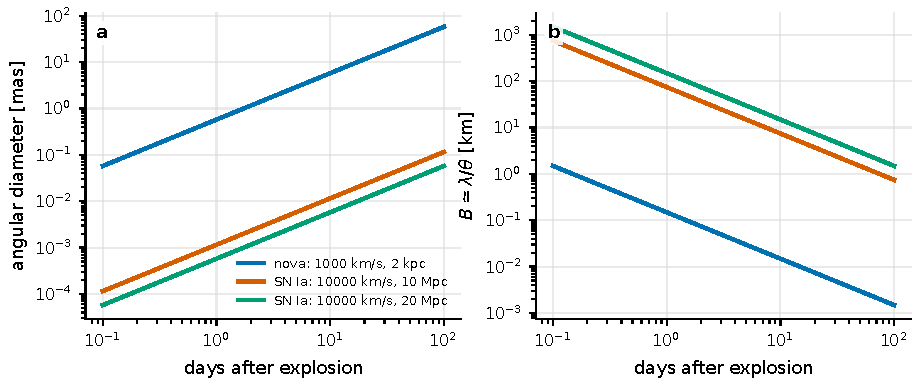
\includegraphics[width=0.94\linewidth]{figures/generated/chapter_19/ch19_transient_expansion.pdf}
\caption{膨胀瞬变的角直径和所需基线。银河系新星在几天到几十天内进入 mas 量级，适合第一代触发演练；10--20 Mpc 的 Type Ia 即使在峰值附近也只有几十微角秒量级，需要 km 级基线和 \(m\lesssim12\) 的近邻事件。}
\label{fig:ch19-transient-expansion}
\end{figure}

Type Ia 强度干涉几何距离是高回报长期目标。Kim 等的可行性研究把 \(m\lesssim12\) 作为可预见下一代观测的亮度范围，对应 \(z\sim0.004\) 的局部体积，预计全天每年约 1 个可用 Type Ia 量级事件。他们用辐射转移模型计算不同波长的表面亮度和 \(|V|^2\)，并指出光谱分辨可以提供多波长层析，测量对象不再局限于一个均匀圆盘半径。第一代项目可以从新星和近邻亮瞬变验证触发、滤光、背景和模型拟合流程；Type Ia 距离标尺应列为二代或专用阵列目标 \citep{2025PhRvD.111h3047K,1997A&A...320..799F,2004A&A...415..531S}。

\section{Crab 光子统计和自然激光怎样检验非热统计}

Crab pulsar 不是空间强度干涉的最佳目标，却是事件表科学的好目标。它亮、周期稳定、有精确星历，光学主脉冲和 interpulse 可以定义相位窗。相位误差为
\begin{equation}
  \Delta\phi
  =
  \frac{\Delta t}{P_{\rm spin}}.
  \label{eq:ch19-pulse-phase}
\end{equation}
\begin{formulaexplain}[公式 (19.7) 解读]
\(\Delta t\) 是时间戳误差，\(P_{\rm spin}\) 是脉冲星自转周期，\(\Delta\phi\) 是相位误差。时间精度越好，事件越能被放进正确的脉冲相位窗。
\end{formulaexplain}
Crab 的 \(P_{\rm spin}\simeq33\,{\rm ms}\)，\(1\,\mu{\rm s}\) 时间误差只对应 \(\Delta\phi\simeq3\times10^{-5}\)；毫秒脉冲星要求更严。AquEYE/Iqueye 这类仪器已经把光子以 ps 到 ns 级时间标签保存，适合做相位分辨 \(g^{(2)}\)、颜色相关或与射电 giant pulse 的条件叠加。Crab giant radio pulse 周期中的光学增强已经被测到，ARCONS 还显示早到的巨脉冲对应更强光学增强；第一代量子天文学可以把这些结果转成事件表统计和偏振/颜色分窗，不必停在平均光变曲线 \citep{2009JMOp...56..261B,2009A&A...508..531N,2015SPIE.9504E..0CZ,2003Sci...301..493S,2013ApJ...779L..12S}。

\begin{figure}[tbp]
\centering
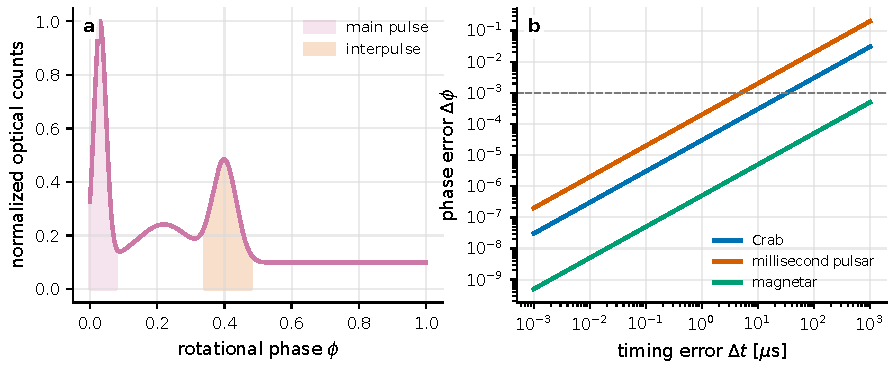
\includegraphics[width=0.94\linewidth]{figures/generated/chapter_19/ch19_crab_phase_windows.pdf}
\caption{Crab 型光学脉冲的相位窗和时间误差。左图示意主脉冲、bridge 和 interpulse 的事件选择；右图把时间误差转成相位误差。对 Crab，微秒级时间已经很宽裕；对毫秒脉冲星，ns--\(\mu\)s 级同步才保留窄相位结构。}
\label{fig:ch19-crab-phase}
\end{figure}

自然激光和受激辐射候选适合做“统计是否非热”的检验；一条亮谱线本身还不够。对 \(M\) 个互不相干热模式，
\begin{equation}
  g^{(2)}(0)-1
  =
  \frac{1}{M},
  \label{eq:ch19-mode-bunching}
\end{equation}
\begin{formulaexplain}[公式 (19.8) 解读]
\(M\) 是互不相干热模式数。模式越多，单模热光的聚束峰越被平均掉；因此 \(g^{(2)}(0)\) 接近 1 不必然说明光是理想激光。
\end{formulaexplain}
而理想相干态给 \(g^{(2)}(0)=1\)。未饱和 maser/laser、饱和放大、自发背景、多斑点叠加和仪器时间响应会产生不同统计。Eta Carinae 的 Weigelt blobs 中 Fe II 线被 Ly\(\alpha\) 泵浦，Johansson 和 Letokhov 讨论了 \(0.9-1.0\,\mu{\rm m}\) 和近红外 Fe II 激光线，线宽测量和 photon-correlation spectroscopy 可作为直接证据。若线宽为 \(\Delta\nu\)，相干时间约 \(\tau_c\sim1/(\pi\Delta\nu)\)；窄线会显著提升可解析相关 contrast，但也要求更高谱分辨、稳定滤光和严格的连续谱扣除 \citep{2004A&A...428..497J,2005NewA...10..361J,2008AIPC..984..216D}。

\begin{figure}[tbp]
\centering
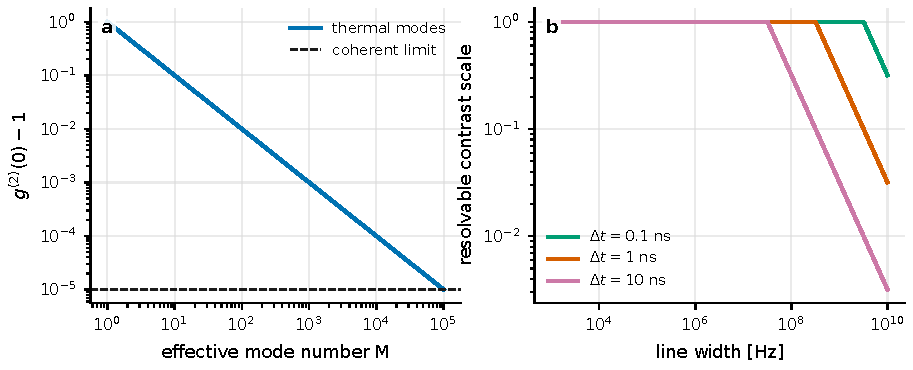
\includegraphics[width=0.94\linewidth]{figures/generated/chapter_19/ch19_natural_laser_statistics.pdf}
\caption{自然激光候选的两个统计量。左图显示热光模式数增加会把聚束峰压低，而相干极限接近 \(g^{(2)}(0)-1=0\)。右图显示线宽越窄，相干时间越长，在给定探测时间分辨率下越容易保留可解析 contrast。}
\label{fig:ch19-natural-laser}
\end{figure}

\section{第一代推荐顺序怎样随仪器成熟变化}

把这些案例放到同一矩阵里，第一代顺序主要由成熟度和系统风险决定。亮热星角直径、已知直径参考星、\(\beta\) UMa 类 A 型星，以及 MAGIC/VERITAS 可重复目标适合作为验收项目。\(\gamma\) Cas 类快速自转、Be/WR 谱线区、密近双星和新星早期膨胀是在同一套能力上继续增加科学信息。Crab 相位分辨统计和自然激光候选线更依赖事件表质量和时间/光谱筛选。Type Ia 几何距离、AGN BLR、暗物质小尺度透镜和量子网络辅助成像科学回报高，但更适合放在长期目标中。

\begin{figure}[!htbp]
\centering
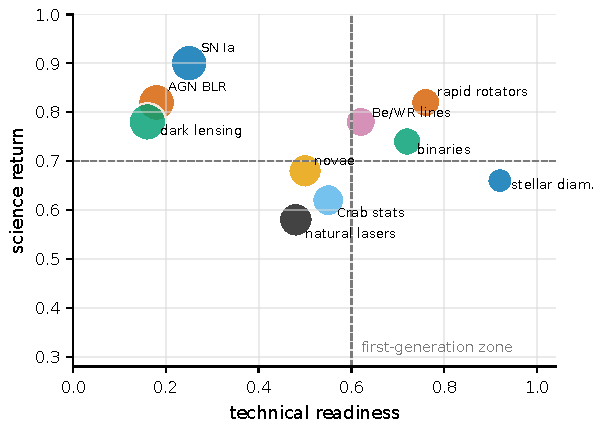
\includegraphics[width=0.78\linewidth]{figures/generated/chapter_19/ch19_priority_matrix.pdf}
\caption{第一代科学案例矩阵。横轴是技术成熟度，纵轴是科学回报，点越大表示系统误差和触发风险越高。右上方且点较小的目标最适合第一代验收；左上方目标科学价值高，但需要专用阵列或更成熟量子资源。}
\label{fig:ch19-priority}
\end{figure}

\begin{longtable}{p{0.17\linewidth}p{0.22\linewidth}p{0.23\linewidth}p{0.20\linewidth}}
\toprule
案例 & 第一观测量 & 典型数量级 & 第一代判据 \\
\midrule
亮星角直径 & \(|V|^2(B)\) & \(m_V<5\)，\(\theta=0.5-2\,{\rm mas}\) & 多夜重复到 \(3-5\%\) 直径精度。 \\
快速自转 & 多位置角 \(|V|^2\) & 轴比 \(1.1-1.5\)，\(\theta<1\,{\rm mas}\) & 能区分圆盘和椭圆模型。 \\
双星 & \(|V|^2\) 振荡 & 分离 \(0.2-5\,{\rm mas}\)，\(f>0.1\) & 已有轨道先验，覆盖两个以上位置角。 \\
Be/WR 谱线 & 谱线/连续谱 \(|V|^2\) & H\(\alpha\)、He、Fe 线 & 线通量足够，连续谱扣除可验证。 \\
新星 & \(\theta(t)\) & 几天后 mas 量级 & 触发快，能与谱线速度合并。 \\
Crab 统计 & 相位窗 \(g^{(2)}\) 和颜色相关 & \(P=33\,{\rm ms}\) & 星历、背景星云和绝对时间闭合。 \\
自然激光 & \(g^{(2)}\)、线宽、偏振 & \(\Delta\nu\) 可窄到高相干时间 & 谱线和连续谱可分离，有 null test。 \\
Type Ia & \(|V|^2(\lambda,t)\) & \(m<12\)，几十 \(\mu{\rm as}\) & km 级阵列和快速触发成熟后再做。 \\
\bottomrule
\end{longtable}

排序会随仪器状态改变。系统刚完成时间同步和零基线相关时，亮星角直径和参考星重复性最有价值；六条以上基线能稳定运行后，快速自转和双星进入主清单；窄带滤光和高数据吞吐可靠后，自然激光和谱线盘才开始有现实空间；阵列扩展到 km 级并能每年快速响应 \(m\lesssim12\) 的瞬变时，Type Ia 几何距离才会成为第一线科学目标 \citep{2017MNRAS.472.4126G,2022MNRAS.512.1722K,2024MNRAS.529.4387A,2024ApJ...966...28A,2025ApJ...995..191A,2025PhRvD.111h3047K}。

